\section{Early warning searches for compact binary coalescence}
\label{SECII}\label{sec:method}

In this section we describe a decomposition of the compact binary parameter
space that reduces low-latency filtering cost sufficiently to allow for the
possibility of \earlywarning\ detection with modest computing requirements.  We
expand on the ideas of~\cite{Marion2004, Buskulic2010} that describe a
multiband decomposition of the compact binary parameter space that resulted in
a search with minutes latency in \LIGO{}'s S6 and Virgo's VSR2 science runs.
We combine this with the \SVD\ rank-reduction method described
in~\cite{Cannon:2010p10398} that exploits the redundancy of the template banks.

\subsection{Conventional \CBC{} matched filter searches}

Inspiral signals are continuously parameterized by a set of intrinsic source
parameters $\vec\theta$ that determine the amplitude and phase evolution of the
gravitational wave strain. For systems where the effects of spin can be
ignored, the intrinsic source parameters are the component masses of the
binary, $\vec\theta = (m_1, m_2)$. Searches for inspiral signals typically
employ matched filter banks that discretely sample the possible intrinsic
parameters~\cite{findchirppaper}.  For a given source, the strain observed by
the detector is a linear combination of two waveforms corresponding to the
`$+$' and `$\times$' gravitational wave polarizations, so for any value of
$\vec\theta$ we must implement 2 filters.  The coefficients for the $\numtmps$ filters
are known as templates, and are formed by discretizing and time reversing the
waveforms and weighting them by the inverse amplitude spectral density of the
detector's noise. To construct a template bank, templates are chosen with the
$\numtmps/2$ discrete signal parameters $\vec\theta_0,\, \vec\theta_1,\, \dots,\,
\vec\theta_{\numtmps/2-1}$ to assure a bounded loss of \SNR~\cite{Owen:1998dk}. That
is, any possible signal within a given range of intrinsic
source parameters will have an inner product that is $\geqslant 0.97$ with at
least one template. Such a template bank is said to have a {\em minimum match}
of 0.97. The data from the detector are whitened and convolved with each
template to produce $\numtmps$ \SNR\ time series. Local peak-finding across time and
templates determines detection candidates.

Filtering the detector data involves a convolution of the data with the
templates.  For a unit-normalized template $h_i[k]$ and whitened detector data
$x[k]$, both sampled at a rate $f^0$, the result can be interpreted as the
signal-to-noise ratio, $\rho_i[k]$ defined as
%
% Filtering equations
%
\begin{equation}
	\label{eq:SNRTD}
	\rho_i [k] = \sum_{n=0}^{N-1} h_{i}[n] x [k-n].
\end{equation}

Equation~(\ref{eq:SNRTD}) can be implemented in the time domain (\TD) as an
\fir\ filter, requiring $\mathcal O(\numtmps \tmpsamps)$ floating point
operations per sample.  However, it is typically much more computationally
efficient to use the convolution theorem and the \fft\ to implement fast
convolution in the frequency domain (\FD), requiring only $\mathcal O(\numtmps
\lg \tmpsamps)$ operations per sample.


\editorial{if we are gonna stick with lloid we should define it}
\subsection{The \lloid\ method}

In the remainder of this section we explore a method for reducing the
computational cost of a \TD\ search for compact binary coalescence.  We will
give a truly zero-latency algorithm that competes in terms of floating point
operations per second with the conventional \FD\ method, which requires a
signficant latency in order to be computationally cheap. Our method, \lloid{},
involves two transformations of the template waveforms that produce a set of
orthogonal filters with far fewer coefficients than the original templates.
The reduction in sample count for all of the filters required to search the
entire parameter space is dramatic.

The first transformation is to chop the time-domain templates up into time
slices.  Since each template slice is disjoint in time, the resulting set for a
single template is orthogonal.  Given the chirp-like structure of the
templates, the early time slices have significantly lower bandwidth and can be
safely downsampled.  The downsampling removes a factor of $\sim 100$ samples
from
%
\editorial{Where do these numbers come from? CHAD: I have actually changed the statement to 100 for the early time slices.}
%
the early part of the waveform and allows the filters to be evaluated at about
$\sim 100$ times lower rate.  This amounts to more than a factor of 10000
reduction in the floating-point operations per second required to filter the
early part of the waveform.  However, the resulting filters are still not
orthogonal across the mass parameter space, and are in fact highly redundant.
We use the singular value decomposition to produce an orthogonal filter set
from the time-sliced templates~\cite{Cannon:2010p10398}.  We find that this
reduces the number of sample points of the filters by another factor of $\sim
100$.  The combined methods reduce the number of floating point operations to
the level where they are competitive with the conventional high-latency \FD\
matched filter approach.  In the remainder of this section we describe the
\lloid\ algorithm in detail and provide some basic computational cost scaling.  

\subsection{Selectively reducing the sample rate of the data and template waveforms}

The first step of our proposed method is to divide the templates into
\emph{time slices} in a time-domain analogue to the frequency-domain
decomposition described in ~\cite{Marion2004, Buskulic2010}.
\editorial{nvf: I've picked the two most relevant; I think they are reasonably complementary.}%
A matched filter is constructed for each time
slice.  The outputs form an ensemble of partial \SNR{} streams.  By linearity,
these partial \SNR\ streams can be suitably time-delayed and summed to
reproduce the \SNR\ of the full template.  To wit,
%
\begin{equation}
\label{eq:time-slices}
h_{i}[k] = \sum_{s=0}^{S-1}
	\cases{%
		h_i^s[k] & for $t^s \leqslant k / f^0 < t^{s+1}$ \\
		0 & otherwise
	}
\end{equation}
%
for $S$ integers $\{f^0 t^s\}$ such that $0  = f^0 t^0 < f^0 t^1 < \cdots < f^0 t^S = N$.
We will show
in the next section that this, combined with the singular value docomposition,
is sufficient to enable a computationally efficient time-domain search and
furthermore is an essential part of an \earlywarning\ detection scheme.

For concreteness and simplicity, we will consider an inspiral waveform in the
quadrupole approximation, for which the time-frequency relation is
%
\begin{equation} \label{eq:fgw}
%
f = \frac{1}{\mathcal{\pi M}} \left[ \frac{5}{256}\frac{\mathcal{M}}{t}
\right]^{3/8}.
%
\end{equation}
%
Here, $\mathcal{M}$ is the chirp mass of the binary in units of time (where $G
M_\odot / c^3 \approx 5 \umu\mathrm{s}$) and $t$ is the time relative to the
coalescence of the binary~\cite{findchirppaper, kidder1992}.  Usually the
template is truncated at some prescribed time $t^0$, or equivalently frequency
$f_\textrm{hi}$.  This is often chosen to correspond to the \ISCO. An inspiral
signal will enter the detection band at a low frequency, $f = f_\mathrm{low}$,
corresponding to a time $t_\mathrm{low}$.  The template is assumed to be zero
outside the interval $[t_\mathrm{low}, t^0)$ and is said to have  a duration of
$t^0 - t_\mathrm{low}$. It is critically sampled at a rate of $2
f_\mathrm{hi}$.

The monotonic time-frequency relationship of equation~\eqref{eq:fgw} allows us
to choose time-slice boundaries that require substantially less bandwidth at
early times in the inspiral.  Our goal is to reduce the filtering cost of a
large fraction of the waveform by computing part of the convolution at a lower
sample rate.  Specifically we consider here time slice boundaries with the
smallest power-of-two sample rate that sub-critically samples the time sliced
template.  The time slices consist of the $S$ intervals $\left(t^S,
t^{S-1}\right],\, \dots,\, \left(t^2, t^1\right],\, \left(t^1, t^0\right]$
sampled at frequencies $f^\mathrm{S-1},\, \dots,\, f^1,\, f^0$ where $f^0
\geqslant 2 f_\mathrm{hi}$ and $f^{S-1} \geqslant 2 f_\mathrm{low}$.  The time
sliced templates may be downsampled without aliasing, so we define them as
%
\begin{equation}
\label{eq:time-sliced-templates}
h_{i}^{s}[k] \equiv
	\cases{
		h_{i}\!\left[k\frac{f}{f^s}\right] & if $t^s \leqslant k/f^s < t^{s+1}$ \\
		0 & otherwise.
	}
\end{equation}
%
\begin{comment}
An example time-slice design satisfying these constraints for a $1.4 - 1.4 \,
M_{\odot}$ binary is shown in table~\ref{table:time_slices}.
%
\begin{table}[h!]
\begin{minipage}[c]{0.52\textwidth}
\centering
\vspace{0.8cm}
\includegraphics{time_slices.pdf}
\end{minipage}
\begin{minipage}[c]{0.3\textwidth}
\centering
\input{time_slices.tex}
\end{minipage}
\caption{\label{table:time_slices} Example of nearly critically sampled,
power-of-two time slices for a $1.4 - 1.4 \, M_{\odot}$ template extending from
$f_\mathrm{low} = 10 \, \mathrm{Hz}$ to $f_\mathrm{hi} = f_\mathrm{ISCO} = 1571\, \mathrm{Hz}$
with a time-frequency structure given by ($\ref{eq:fgw})$. $f^s$ is the sample
rate of the time slice, $(t^{s+1}, t^s]$ are the boundaries in seconds
preceeding coalescence and \slicessamps\ is the number of samples in the
$s^{\mathrm{th}}$ filter.}
\end{table}
\end{comment}

Since waveforms with neighboring intrinsic source parameters $\vec\theta$ have
similar time-frequency evolution, it is possible to design computationally
efficient time slices for an extended region of parameter space rather than to
design different time slices for each template.

We note that the time slice decomposition in equation~(\ref{eq:time-slices}) is
manifestly orthogonal since the time slices are disjoint in time.  In the next
section we examine how to reduce the number of filters within each time slice
via singular value decomposition of the time sliced templates.

\subsection{Reducing the number of filters with the singular value
decomposition}

As described previously, the template banks are, by design, highly correlated.
It is possible to greatly reduce the number of filters required to achieve a
particular minimum match by designing an appropriate set of \SVD\ {\em
basis templates}.  A numerical technique based on the singular value
decomposition (\SVD) of inspiral template banks is demonstrated
in~\cite{Cannon:2010p10398}.  Similarly, the time sliced templates described
above can be approximated to arbitrary accuracy by expansion into a set of
\SVD\ \emph{basis templates}, $u_l^s[k]$, related to the original time
sliced templates through the \emph{reconstruction matrix},
$v_{il}^s\sigma_l^s$:
%
\begin{equation}
h_i^s[k] = \sum_{\mathclap{l=0}}^{\mathclap{M-1}} v_{il}^s \sigma_l^s u_l^s[k] \approx \sum_{\mathclap{l=0}}^{\mathclap{L^s-1}} v_{il}^s \sigma_l^s u_l^s[k].
\label{eq:svddecomp}
\end{equation}
%
\editorial{Say a word or two about \SVD\ tolerance?}%
%
The parameter $\numsvdtmps$ sets the number of basis templates that are kept in
the approximation.  This determines the \SVD\ tolerance, which affects the
\SNR\ loss due to the approximation.  The authors of \cite{Cannon:2010p10398}
showed that high accuracy could be achieved with far fewer basis templates than
templates in the original template bank.  We find that when combined with the
time-slice decomposition, the number of basis templates \numsvdtmps\ is much
smaller than the original number of templates \numtmps.  In the next section we
describe how we form our novel detection statistic using the time-slice
decomposition and the \SVD.

\subsection{Early warning \SNR }

In the previous two sections we have described two transformations that greatly
reduce the burden of filtering the compact binary parameter space and make \TD\
filtering of the data possible.  We are now prepared to define the early
warning \SNR\ and to comment on the computational cost of evaluating it.  But
first, we will introduce some notation refering to the decimation of data,
which means reducing the sample rate after low-pass filtering,
\begin{equation}
\label{eq:decomp}
	x^{s+1}[k] = \left( H^\shortdownarrow x^s\right)[k] \,,
\end{equation}
and notation refering to the interpolation of data to increase the sample rate,
\begin{equation}
	x^{s}[k] = \left( H^\shortuparrow x^{s+1}\right)[k] \,.
\end{equation}

From the combination of transformations to the compact binary templates defined
in equation \eqref{eq:time-sliced-templates} and \eqref{eq:svddecomp} we define
the early-warning filter output accumulated up to time slice $s$ as,
%
% orthogonal decomposition filtering
%
\begin{equation}
	\rho_i^s [k] =%
		% Reconstruction
		\underbrace{
			\sum_{\mathclap{l=0}}^{\mathclap{L^s-1}} v_{il}^s \sigma_l^s
		}_\textrm{\clap{reconstruction}}
		% Orthogonal FIR filter
		\overbrace{
			\sum_{\mathclap{n=0}}^{\mathclap{N^s-1}} u_l^s[n] x^s[k-n]
		}^\textrm{\clap{orthogonal {\sc fir} filters}}
		% Plus ...
		+
		% Interpolation SNR
		\underbrace{
			\left(H^\uparrow \rho_i^{s+1}\right)[k]
		}_\textrm{\clap{{\sc snr} from previous time slices}}
\end{equation}
%
%
\FIXME{This quantity is related to the early warning \SNR{} by the normalization
of the partial filter defined by the present time slice.}
%
%
\begin{figure}[htbp]
	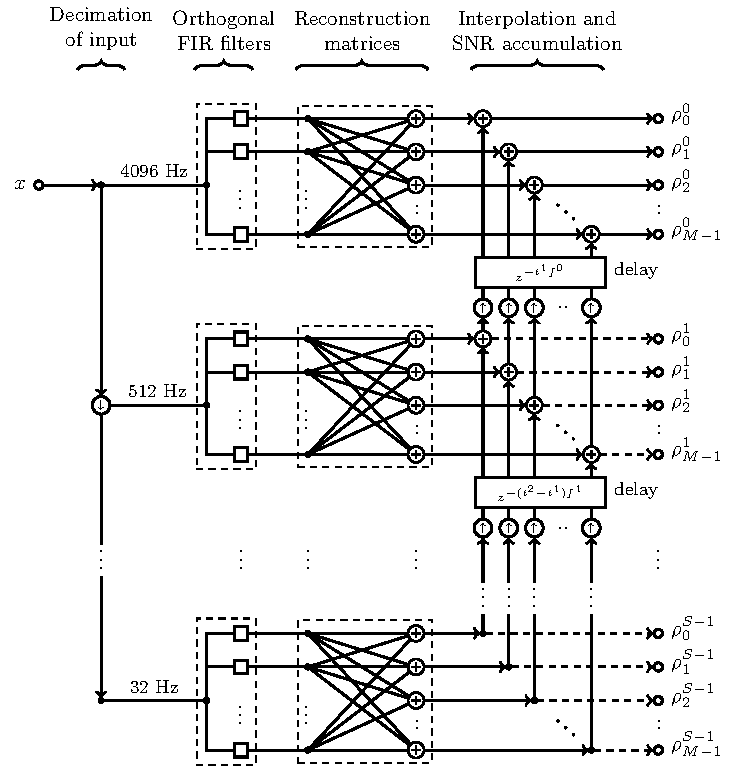
\includegraphics{figures/lloid-diagram.pdf}
	\caption{\label{fig:pipeline} Schematic of \lloid{} pipeline illustrating
signal flow.  Circles with arrows represent interpolation
\protect
\includegraphics{figures/upsample-symbol.pdf} or decimation
\protect
\includegraphics{figures/downsample-symbol.pdf}.  Circles with plus
signs represent summing junctions
\protect
\includegraphics{figures/adder-symbol.pdf}.  Squares
\protect
\includegraphics{figures/fir-symbol.pdf} stand for \fir{} filters.  Sample
rate decreases from the top of the diagram to the bottom.  In this diagram each
time slice contains three \fir\ filters that are linearly combined to produce
four output channels.  In a typical pipeline the number of \fir\ filters is
much less than the number of output channels.}
\end{figure}
%
%
The signal flow diagram in figure~\ref{fig:pipeline} illustrates how this
recursion relation can be realized as a multirate filter network with outputs for
each of the early warning \SNR{}s.

In the next section we compute the expected computational cost scaling of this
decomposition and compare it with the brute-force time-domain implementation of
\eqref{eq:SNRTD} and higher latency frequency-domain methods.

\subsection{Comparison of computational costs}

We now examine the computational cost scaling of the approximate implementation
of a conventional time-domain or frequency-domain matched filter bank as compared
with \lloid{}.  For convenience, table~\ref{tab:recap} provides a review of the notation
that we will need in this section.
%
% symbols used in FLOPs calculations table
%
\Table{\label{tab:recap} Notation used to describe filters.}
\br
	& Definition \\
\mr
\numtmps		& number of templates \\
\tmpsamps	& number of samples per template \\
\numslices	& number of time slices \\
\numsvdtmps	& number of orthogonal templates in time slice $s$ \\
\slicessamps	& number of samples in time slice $s$ \\
$f^s$		& sample rate in time slice $s$ \\
$N^\shortdownarrow$ & number of coefficients in decimation filter \\
$N^\shortuparrow$ & number of coefficients in interpolation filter \\
\br
\end{tabular}
\end{indented}
\end{table}

\editorial{This section's two tables are small.  Any way to put them side by side or next to another figure?}

\Table{\label{table:flops}Minimum computational cost of the \fir{} filter bank, \fft{} convolution, and \lloid\ methods for a bank of 657 templates sampled at 4096 Hz.}
\br
Method & \flops \\
\mr
\fir{} & $2.4\times10^{13}$ \\
\fft{} convolution & $2.6\times10^8$ \\
\lloid & $4.7\times10^8$ \\
\br
\end{tabular}
\end{indented}
\end{table}

\subsubsection{Conventional time-domain method}

The conventional time-domain method consists of a bank of \fir{} filters, or sliding-window dot products.  If there are $\numtmps$ templates, each $\tmpsamps$ samples in length, then each filter requires $M N$ multiplications and additions per sample, or $2 \numtmps \tmpsamps f^0$ floating point operations per second (\flops) at a sample rate $f^0$.

\subsubsection{Conventional frequency-domain method}

The most common frequency-domain method is known as the \emph{overlap-save} algorithm, described in \cite{numerical-recipes-chapter-13}.  It entails splitting the input into blocks of $D$ samples, $D > \tmpsamps$, each block overlapping the previous one by $D - \tmpsamps$ samples.  For each block, the algorithm computes the forward \fft\ of the data and the templates, multiplies them, and then computes the reverse \fft.

Modern implementations of the \fft, such as the ubiquitous \texttt{fftw}, require about $2 \fftblock \lg \fftblock$ operations to evaluate a real transform of size $\fftblock$~\cite{Johnson:2007p9654}.  Including the forward transform of the data and $M$ reverse transforms for all of the templates, the \fft\ costs $2 (\numtmps + 1) \fftblock \lg \fftblock$ operations per block.  The multiplication of the transforms adds a further $2 \numtmps \fftblock$ operations per block.  Since each block produces $\fftblock - \tmpsamps$ usable samples of output, the overlap-save method requires
$$
f^0 \cdot \frac{2 (\numtmps + 1) \lg \fftblock + 2 \numtmps}{1 - \tmpsamps/\fftblock} \; \mathrm{\flops}.
$$

\subsubsection{\lloid\ method}

For time slices $s$, the \lloid\ method requires $2 \slicessamps \numsvdtmps f^s$ \flops\ 
for evaluating the orthogonal filters, $2 \numtmps \numsvdtmps f^s$ \flops\ for the 
linear transformation from the $\numsvdtmps$ basis templates to the $\numtmps$ time-sliced templates, and $\numtmps f^s$ \flops\ to add the resultant partial \SNR\ stream.

The computational cost of the decimation of the detector data is a little bit more subtle.  Decimation is achieved by applying an \fir\ antialiasing filter and then downsampling, or deleting samples in order to reduce the sample rate from $f^{s-1}$ to $f^s$.  Naively, an antialiasing filter with $N^\shortdownarrow$ coefficients should demand $2 N^\shortdownarrow f^{s-1}$ \flops.  However, it is necessary to evaluate the antialiasing filter only for the fraction $f^s / f^{s-1}$ of the samples that will not be deleted.  Consequently, an efficient decimator that requires only $2 N^\shortdownarrow f^{s-1} \cdot \left( f^s / f^{s-1} \right) = 2 N^\shortdownarrow f^s$ \flops\ is possible.

The story is similar for the interpolation filters used to change the sample rates of the partial \SNR{} streams.  Interpolation of a data stream from a sample rate $f^s$ to $f^{s-1}$ consists of inserting zeros between the samples of the original stream, and then applying a low-pass filter with $N^\shortdownarrow$ coefficients.  The low-pass filter requires $2 M N^\shortdownarrow f^{s-1}$ \flops.  However, by taking advantage of the fact that by construction a fraction $f^{s-1}/f$ of the samples are zero, it is possible to build an efficient interpolator that requires only $M N^\shortuparrow f^{s-1} \cdot \left( f^s / f^{s-1} \right) = 2 M N^\shortuparrow f^s$ \flops.

Taking into account the decimation of the detector data, the orthogonal \fir\ filters, the reconstruction of the time-sliced templates, the interpolation of \SNR\ from previous time slices, and the accumulation of \SNR, in total \lloid\ requires
$$
\sum_{\mathclap{s=0}}^{\mathclap{S-1}} \left( 2 \slicessamps \numsvdtmps + 2 \numtmps \numsvdtmps + \numtmps \right) f^s + 2\sum_{\mathclap{f \in \{f^s\}}} \left( N^\shortdownarrow + \numtmps N^\shortuparrow \right) f \textrm{ \flops.}
$$
The second sum is carried out over the set of sample rates of all of the time slices rather than over the time slices themselves because some time slices may have the same sample rates.

\subsubsection{Extrapolation of the computational cost to an Advanced LIGO search}

Table~\ref{table:flops} shows that the \lloid\ method requires $\sim 10^8$ \flops\
to cover a sub-bank of comprising $\sim 10^2$ out of $\sim 10^5$ sets of intrinsic
source parameters.  Given that modern (ca. 2011) workstations can sustain
computation rates up to $\sim 10^{10}$ \flops{}, and assuming that other regions of the
parameter space have similar computational scaling, an entire search could be implemented
with $\gtrsim 10$ machines.

By comparison, using the \TD\ method to achieve the same latency costs $\sim 10^{13}$ \flops\ for this particular sub-bank, and so it would require $\sim 10^6$ present-day machines.  Presently, the \LIGO\ data grid consists of only $\sim 10^4$ machines.

\begin{comment}

% Do we want to spend this much copy on the whitener?
% What matters is that we have picked a low-latency whitening procedure.

\subsection{Data Whitening}
Matched filtering the SVD basis vectors has motivated a decoupling of the
whitening routine from the matched filtering engine. This was necessary in
order weight templates appropriately by whitening them before the SVD
calculation, and, as such, we have also moved the data whitening outside the
match filter engine. We have chosen to whiten the data using a running
geometric average of the PSD computed by Hann windowing 8 second buffers of
data and using 50\% overlapping buffers. The running geometric average is
updated once per buffer from a median of the recent PSDs. We find that this
algorithm is extremely fast to converge to an accurate PSD and also very robust
against glitches.

An inspiral, to leading order, has gravitational-wave frequency evolution given
by
%
\begin{equation}
%
f(t) = \frac{1}{8 \pi \mathcal{M}} \left( \frac{t_c - t}{5 \mathcal{M}}
\right)^{-3/8}\;,
%
\end{equation}
%
whose time derivative is given by
%
\begin{equation}
%
\frac{df}{dt} = \frac{3}{320 \pi \mathcal{M}^2} \left( \frac{t_c - t}{5
\mathcal{M}} \right)^{-11/8}\;.
%
\end{equation}
%
Combining these, we find the frequency evolution as a function of frequency to
be
%
\begin{equation}
%
\frac{df}{dt}(f_0) = \frac{3}{320 \pi \mathcal{M}^2} \left( 8 \pi \mathcal{M}
f_0 \right)^{3/11}\;,
%
\end{equation}
%
which can be inverted to get the minimum frequency which has a given frequency
derivative,
%
\begin{equation}
%
f_0 = \frac{1}{8 \pi \mathcal{M}} \left( \frac{320 \pi \mathcal{M}^2}{3}
\frac{df}{dt} \right)^{11/3}\;.
%
\end{equation}

If we allow frequency bins to be affected by an injection only once within the
median history, we need to calculate the corresponding $df/dt$ for our PSD
calculation. An FFT of a buffer with length $T$ will have a frequency
resolution $df = 1/(2T)$. Hann windowing the data and overlapping buffers by
50\% introduces correlations in neighboring frequency bins of the FFT. This
means that we actually want the frequency to change by $df = 3/(2T)$ before the
next PSD calculation, which happens a $dt = T/2$ later, resulting in a minimum
$df/dt = 3/T^2$.

Combining these results we find the lower frequency bound for our injections,
assuming a chirp mass for a binary with $m_1 = m_2 = 1 M_{\odot}$ and $T = 8$
s, is 23 Hz.

We want to compute the equivalent injection density which would be biased as
much as lalapps\_inspiral's PSD estimator, which allows $\sim3$ injections per
2048 seconds. It computes the PSD by breaking the segment up into 16 256 second
chunks. These chunks are then combined into to sets of 8 chunks each. The
median of each set is then averaged across the sets for each frequency bin to
produce the PSD estimate for that 2048 second segment. This procedure results
in an average injection density of 1.5 per 8 PSDs in the median history, which
is comparable to LLOID's 1 per 7 PSDs in the median history. Since LLOID has an
injection history of 7 PSDs which span 32 seconds, this means LLOID can perform
one injection every 32 seconds, or 64 injections per 2048 second segment, more
than an order of magnitude increase in density over lalapps\_inspiral.
\end{comment}
